\chapter{Nintendo Entertainment System ismertetése}

A Nintendo Entertainment System (NES) egy otthoni videojáték-konzol, amelyet a Nintendo 1983-ban Japánban (Family Computer, röviden FamiCom néven) és 1985-ben Észak-Amerikában, Európában és Ausztráliában adott ki. Ez minden idők egyik legikonikusabb és legnagyobb hatású videojáték-konzolja.

A NES döntő szerepet játszott a videojáték-ipar újjáélesztésében az 1983-as észak-amerikai videojáték-válság után. Számos klasszikus és kedvelt játékot mutatott be, amelyeket a játékosok még ma is nagyra tartanak. A konzol sikere az erős játéktárnak, a felhasználóbarát kialakításnak és az innovatív marketingstratégiáknak köszönhető.
%TODO kép a konzolról
\begin{figure}[H]
	\centering
	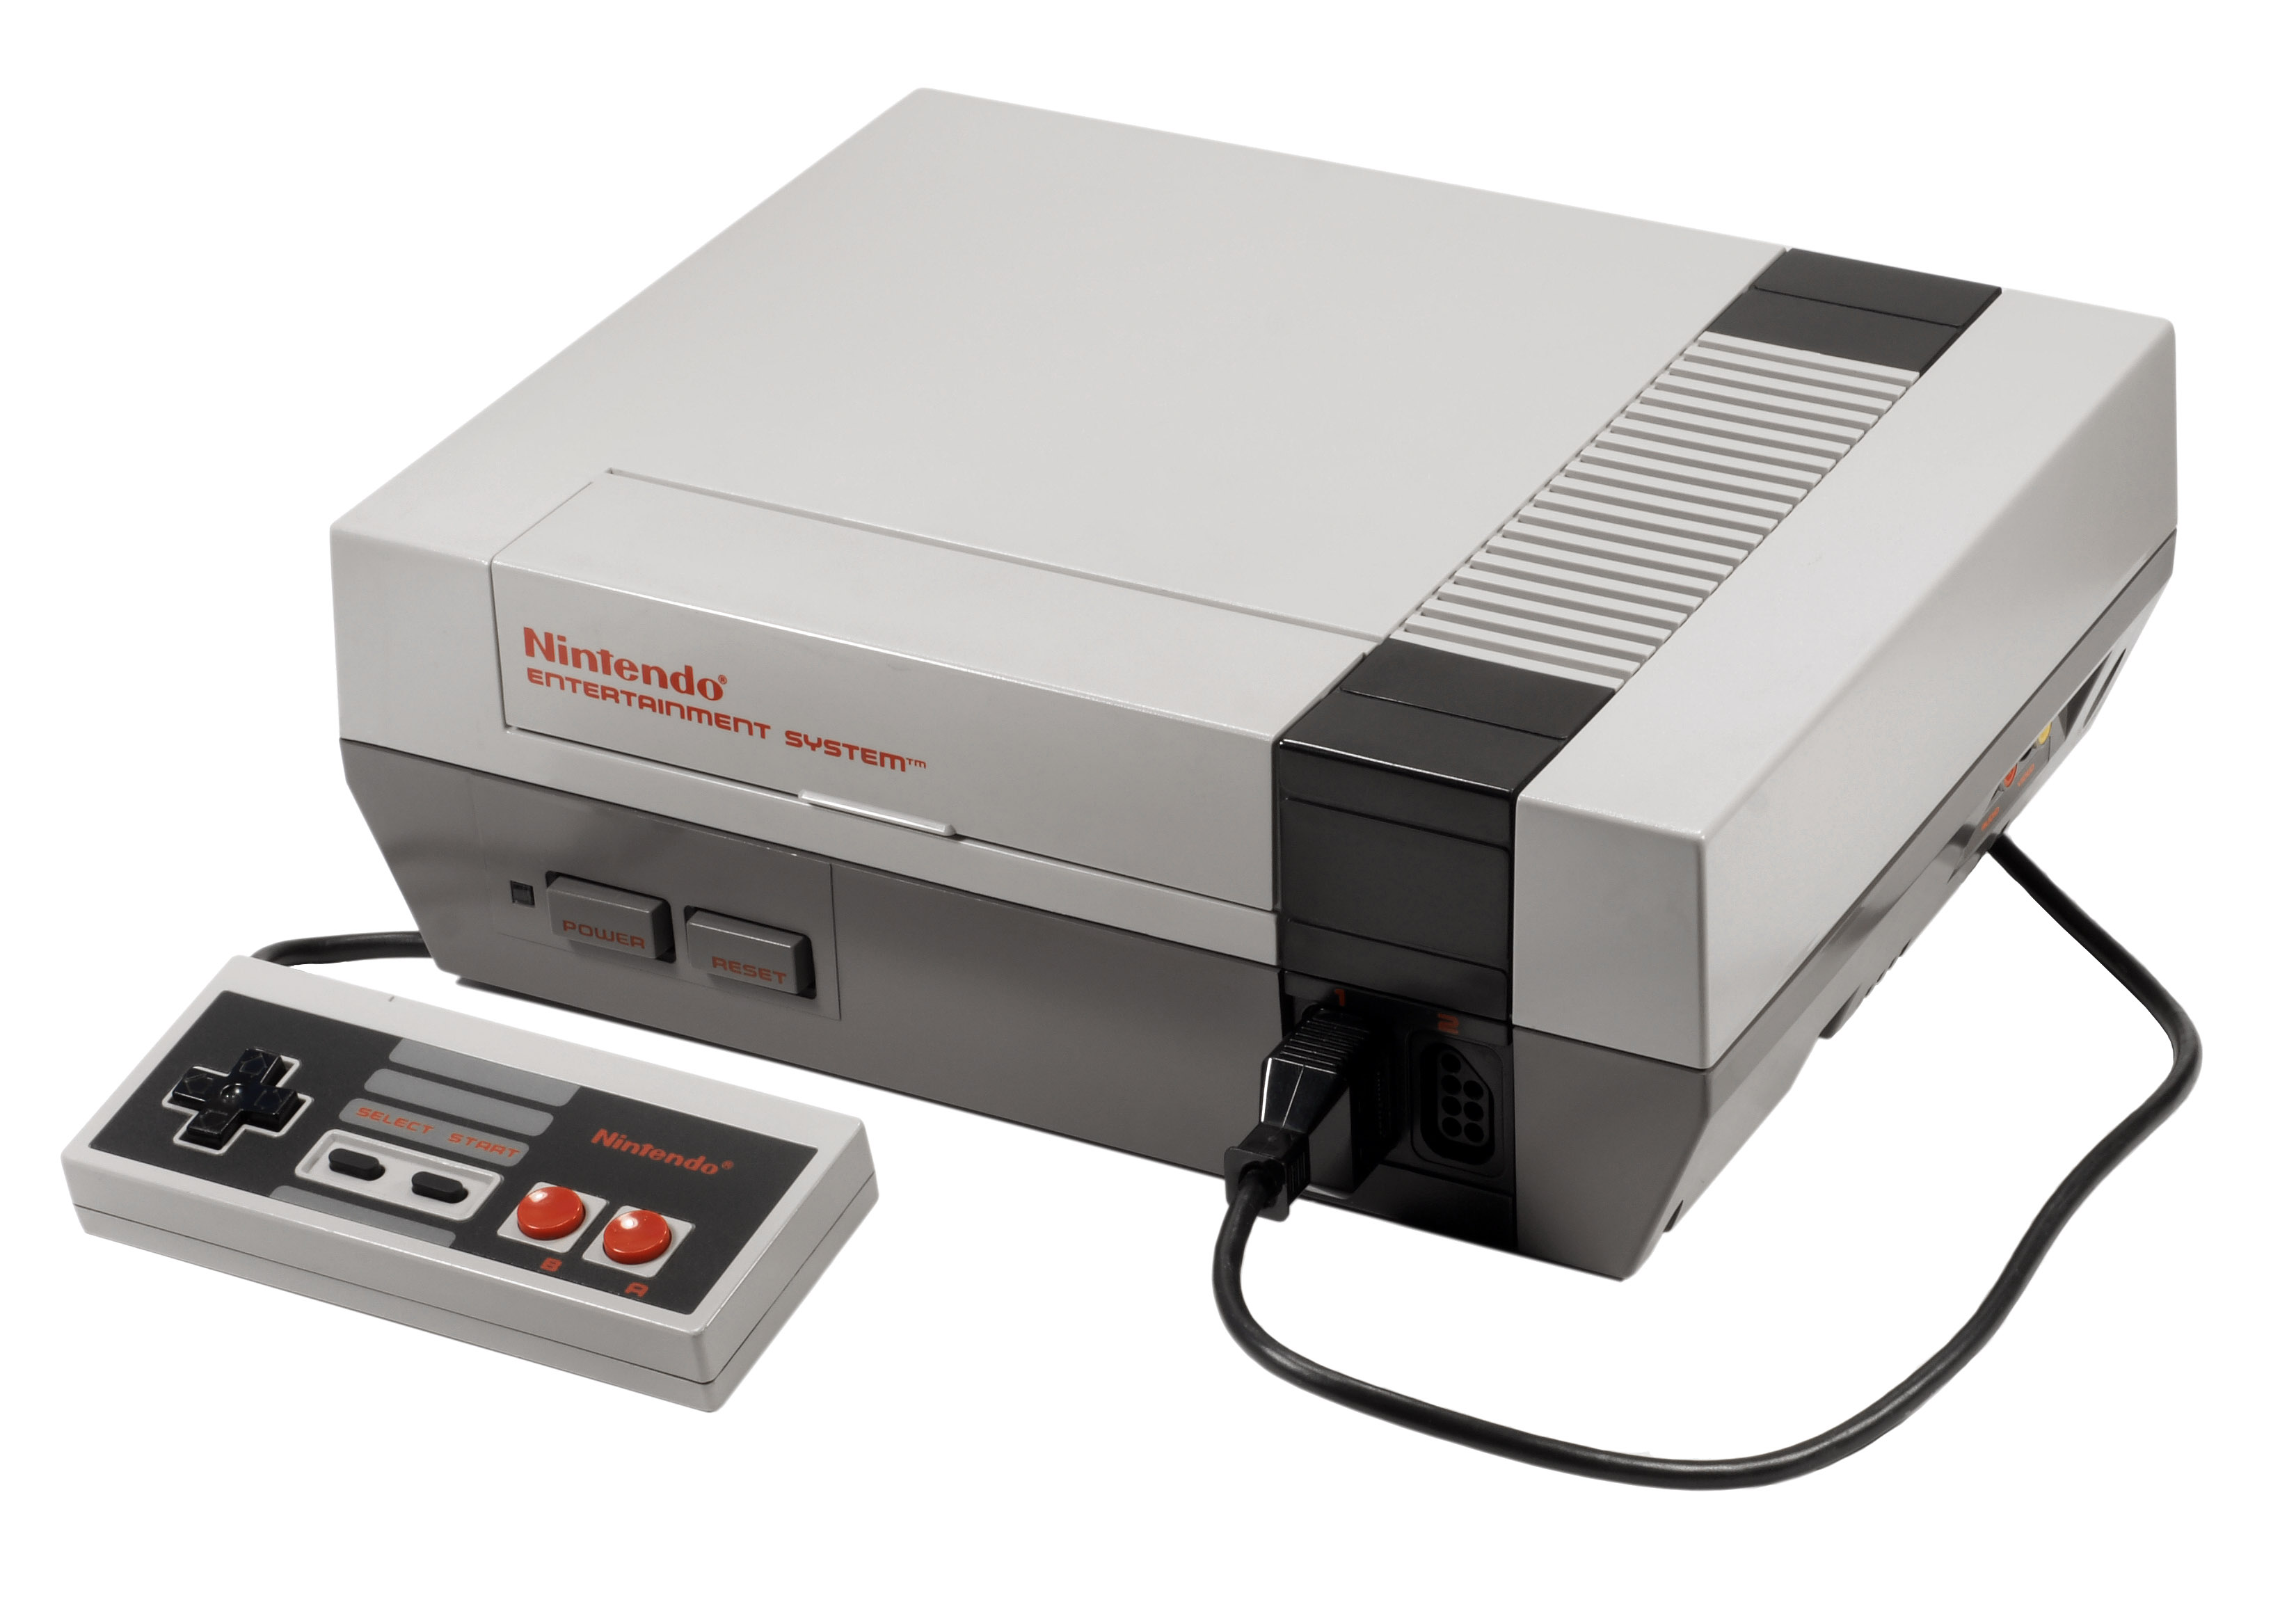
\includegraphics[width=120mm, keepaspectratio]{figures/NES-console-set}
	\caption{Nintendo Entertainment System}
	\label{fig:NES-Consol}
\end{figure}

Az otthoni konzol 8 bites processzorral rendelkezett, és a játékok tárolására elsősorban kazettákat használt. Jellegzetes, téglalap alakú kialakítása volt, a játékkazetták behelyezésére szolgáló elülső betöltő mechanizmussal. A konzolhoz egy pár kontroller is tartozott, és bevezette a ma már ikonikus NES kontroller kialakítását, amely irányjelzővel, start- és választógombokkal, valamint az A és B gombokkal rendelkezett.

A konzolra megjelent legnépszerűbb és legnagyobb hatású játékai közé tartozik a Super Mario Bros., a The Legend of Zelda, a Metroid, a Mega Man, a Castlevania és még sok más játék. Ezek a játékok megalapoztak számos sikeres franchise-t, amelyek ma is virágoznak.

A játékkonzol hardverének megismerésére, elsősorban a hivatalos wiki oldalt használtam. Az itt olvasható tartalmakat az évek során nagy részt az eredeti hardver visszafejtésével (reverse engineering) tárták fel, mivel a játékkonzol pontos adatlapjai, illetve időzítés és működési diagramjai nem lettek publikusak (a Nintendo tulajdonban vannak). Az oldalon szereplő adatokat a NESDev online közösség tartja karban, ezáltal az oldal pontos és helyes adatokat tartalmaz (ezeket a közösség rendszeresen felül vizsgálja). A NES eredeti hardverének áttekintéséhez és a chippek megismeréséhez (PPU, CPU) nagy segítséget nyújtott még a NESHacker youtube csatorna. 

\section{NES hardver főbb komponensei}

A Nintendo Entertainment System hardverének áttekintéséhez célszerű az eredeti konzol alaplapjának tüzetes vizsgálata. Ezt \aref{fig:NES-Motherboard} képen láthatjuk, és ez alapján a komponensek öt fő csoportba sorolhatjuk.

\begin{figure}[H]
	\centering
	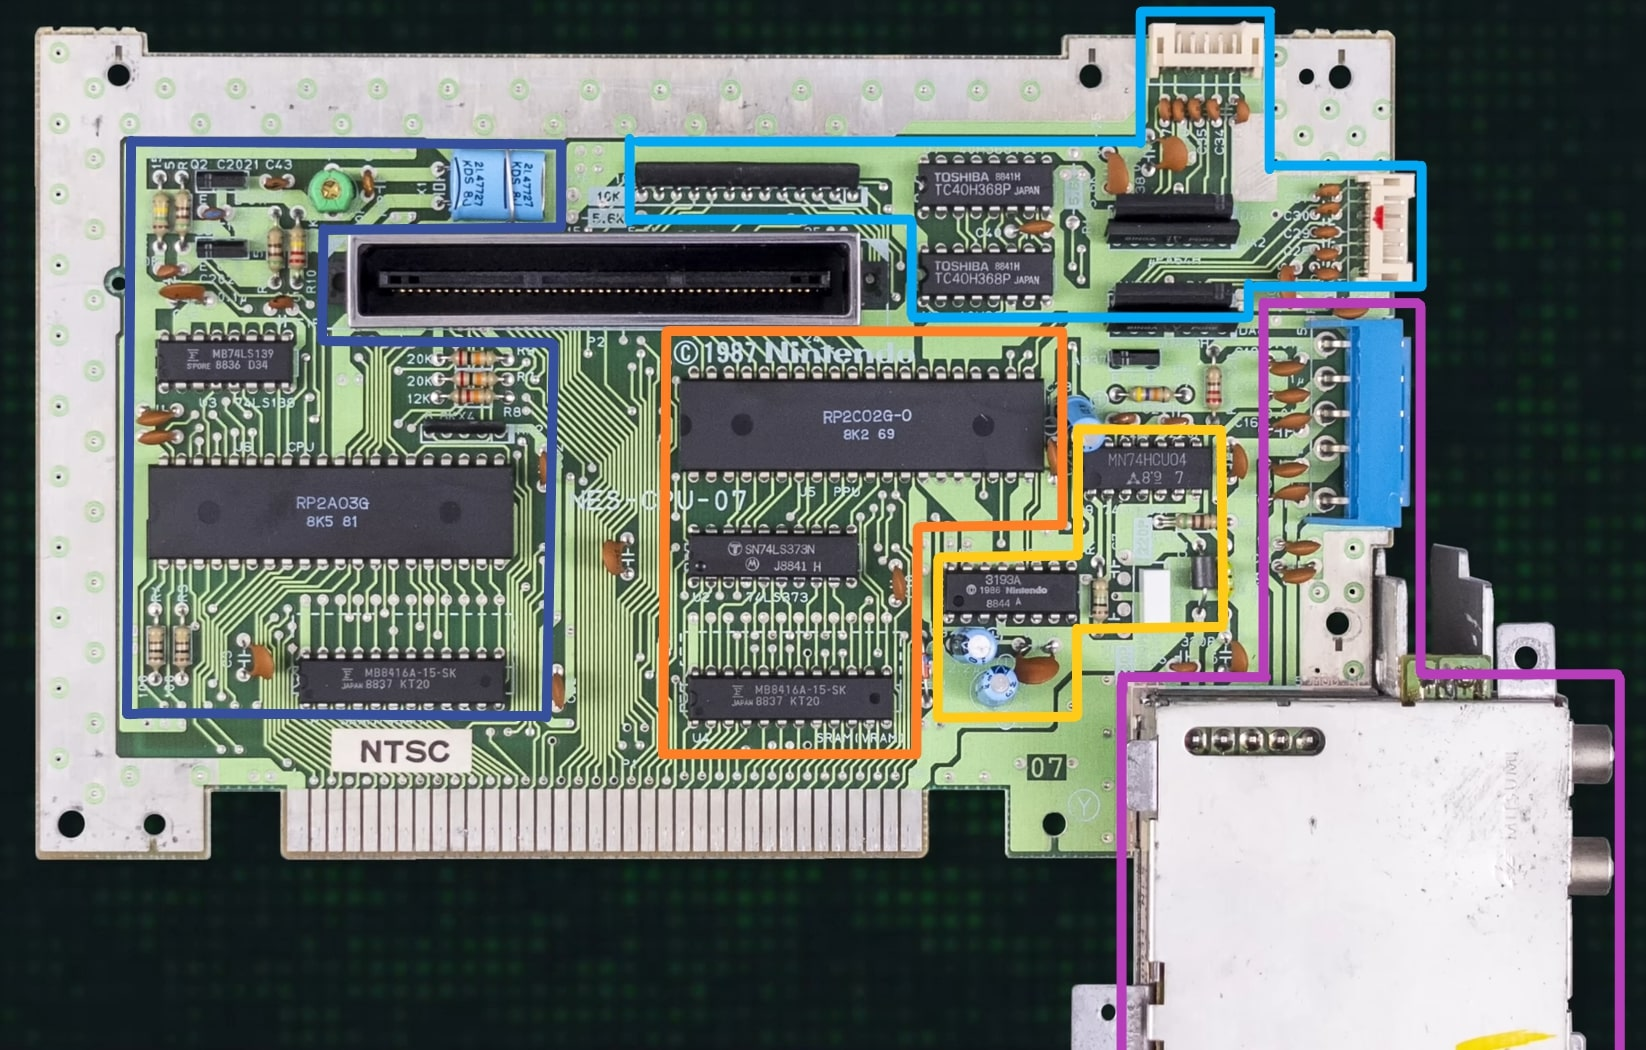
\includegraphics[width=150mm, keepaspectratio]{figures/NES-motherboard-lines}
	\caption{Nintendo Entertainment System NTSC alaplap \cite{NES_hardware}}
	\label{fig:NES-Motherboard}
\end{figure}

\begin{itemize}
	\item \emph{Sötétkék, processzor:} A NES processzora és ennek kiegészítő áramkörei, komponensei. Ide tartozik természetesen az RP2A03G chip, ez a fő vezérlő egyég két fő elemet tartalmaz : egy átalakított 6502-es processzort, illetve az APU co-processzort amely a hang generálásért felelős. Ezen a kék területen belül még megtalálható a WRAM (cpu alatt) amely egy két kilobájt méretű rendszer memória (system memory) ként volt használva, illetve az 74LS139-is (cpu-tól balra fent) amely a chip kiválasztó (chip select) jelek elő állításáért felelős hardver. Itt kapott még helyet a keret tetején látható kék oszcillátor kristály is és ennek segéd áram köre. Ez a komponens látta el az egész alaplapot órajellel.
	\item \emph{Narancssárga, videó generálás:} Ebbe a kategóriába három komponens tartozik. Első az RP2C02G-O chip amely a videó generálás fő vezérlő egysége volt, ennek neve Picture Process Unit (PPU). A PPU alatt pedig a két memória chip látható, az alsó raktározta el a képgeneráláshoz szükséges adatokat (VRAM), a fölötte lévő egy adatpufferként funkcionált.
	\item \emph{Citromsárga, CIC chip:} Itt található a CIC chip amely azért volt felelős, hogy nem licencelt játékokat ne lehessen a NES-el játszani. Illetve itt még egy invertáló áramkör kapott helyet (ezt nagyjából minden alaplapi komponens használta ha bit invertálásra volt szüksége). 
	\item \emph{Lila, kompozit kimenet:} Ezen a területen láthatók a kompozit jel elő állításáért felelős áramköri elemek és a táp bemenet szűrésért felelős kapacitások.
	\item \emph{Világoskék, kontrollerek:} A fenti csatlakozó az egyes játékos kontroller portja a jobb oldali pedig a második játékosé. Itt még látható két dedikált invertáló komponens is, amelyek a kontrollerekből érkező adatok negálásával foglalkoztak.
\end{itemize}

A fenti elemek kívül az alaplapon még található középen egy bővítő csatlakozó is, illetve a kártya aljára lehet közvetlenül csatlakoztatni a játék kazettákat is. A játék kazetták multifunkcionális nyákok voltak és általában \aref{fig:NES-Game-Cartridge} ábrán látható módon néztek ki. 

\begin{figure}[H]
	\centering
	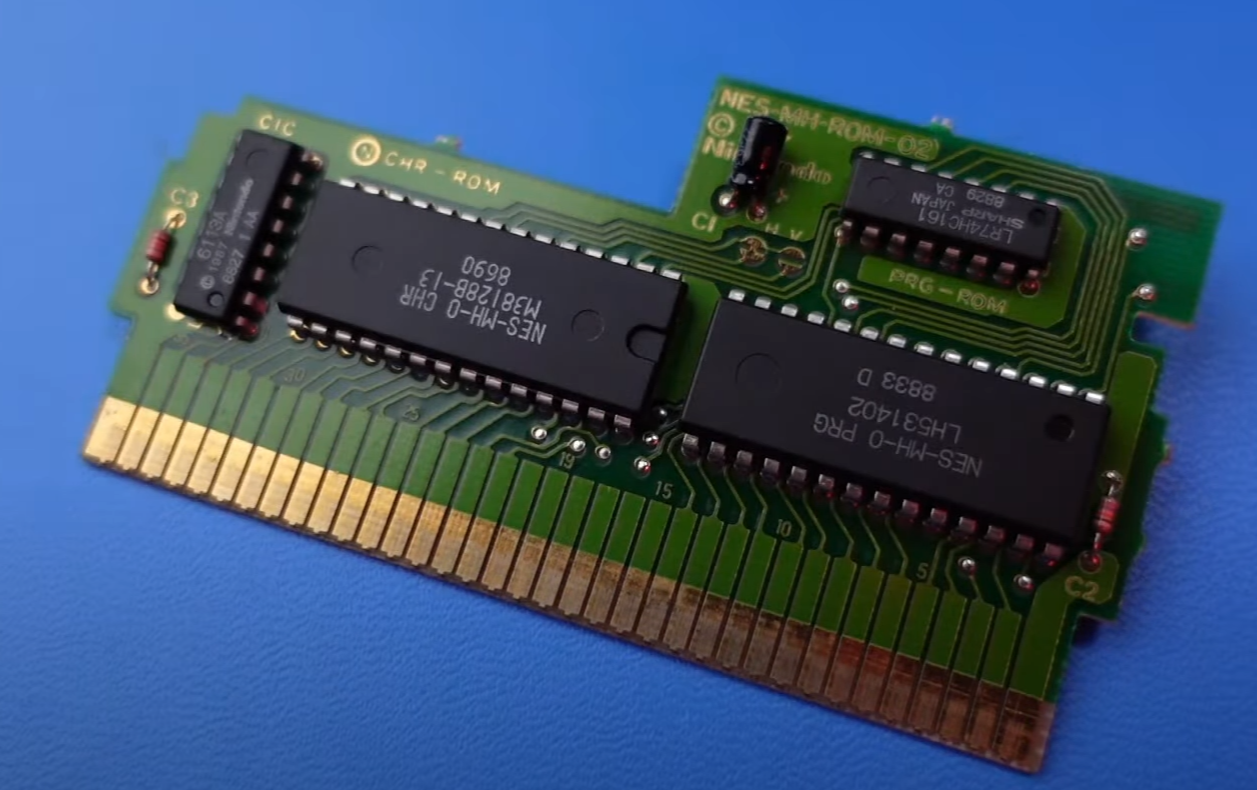
\includegraphics[width=150mm, keepaspectratio]{figures/Mario-Duckhunt-cartage}
	\caption{Nintendo Entertainment System játék kazetta \cite{NES_cartridge}}
	\label{fig:NES-Game-Cartridge}
\end{figure}

A  játék kazetták fő alkotó elemei:

\begin{itemize}
	\item \emph{Program ROM, és Mapper-ek:} A játék szoftvert tartalmazó, kezdetben 16 kilobájt - 32 kbyte méretű ROM. Viszont a 32 kilobájtnál nagyobb játékok esetén a ROM egy extra segéd chippel (Mapper) egészült ki, amelyen keresztül a NES megtudta címezni a nagyobb ROM területet. 
	\item \emph{Karakter ROM:} Általában 8 kilobájt méretű ROM. A megjelenítéshez szükséges csempe elemeket tárolja (\ref{fig:Mario-Pattern}).
	\item \emph{CIC chip:} Ez a komponens licencelte a játék szoftverét a NES konzol felé.
\end{itemize}

	\subsection{Komponensek kapcsolata - PPU és CPU adatbusz}
	
	A különböző komponensek mélyebb bemutatása előtt a NES hardverének adat kapcsolatát is át kell tekintenünk. A NES úgynevezett memory-mapped I/O architektúrával rendelkezik. Ez egy olyan technika amely a rendszer teljes memória területét feldarabolja nagyobb egységekre, és ezeket hardveres komponensekhez rendel. Ezek alapján az alaplapon található WRAM, a játék kártyán található Program ROM, illetve a PPU hét vezérlő regisztere és az APU vezérlőregisztere, mind a CPU 16 bites címterületén belül található és a CPU adatbuszon keresztül írható és olvasható. A NES-en belül található még egy PPU adatbusz is amely a VRAM-ot és a játék kazettán található karakter ROM-ot foglalja a PPU cím tartományba (\ref{tab:PPU-memory}). Ezeket az adatkapcsolatokról \aref{fig:NES-Data-Buses} sematikus ábra foglalja össze.
	
	\begin{figure}[H]
		\centering
		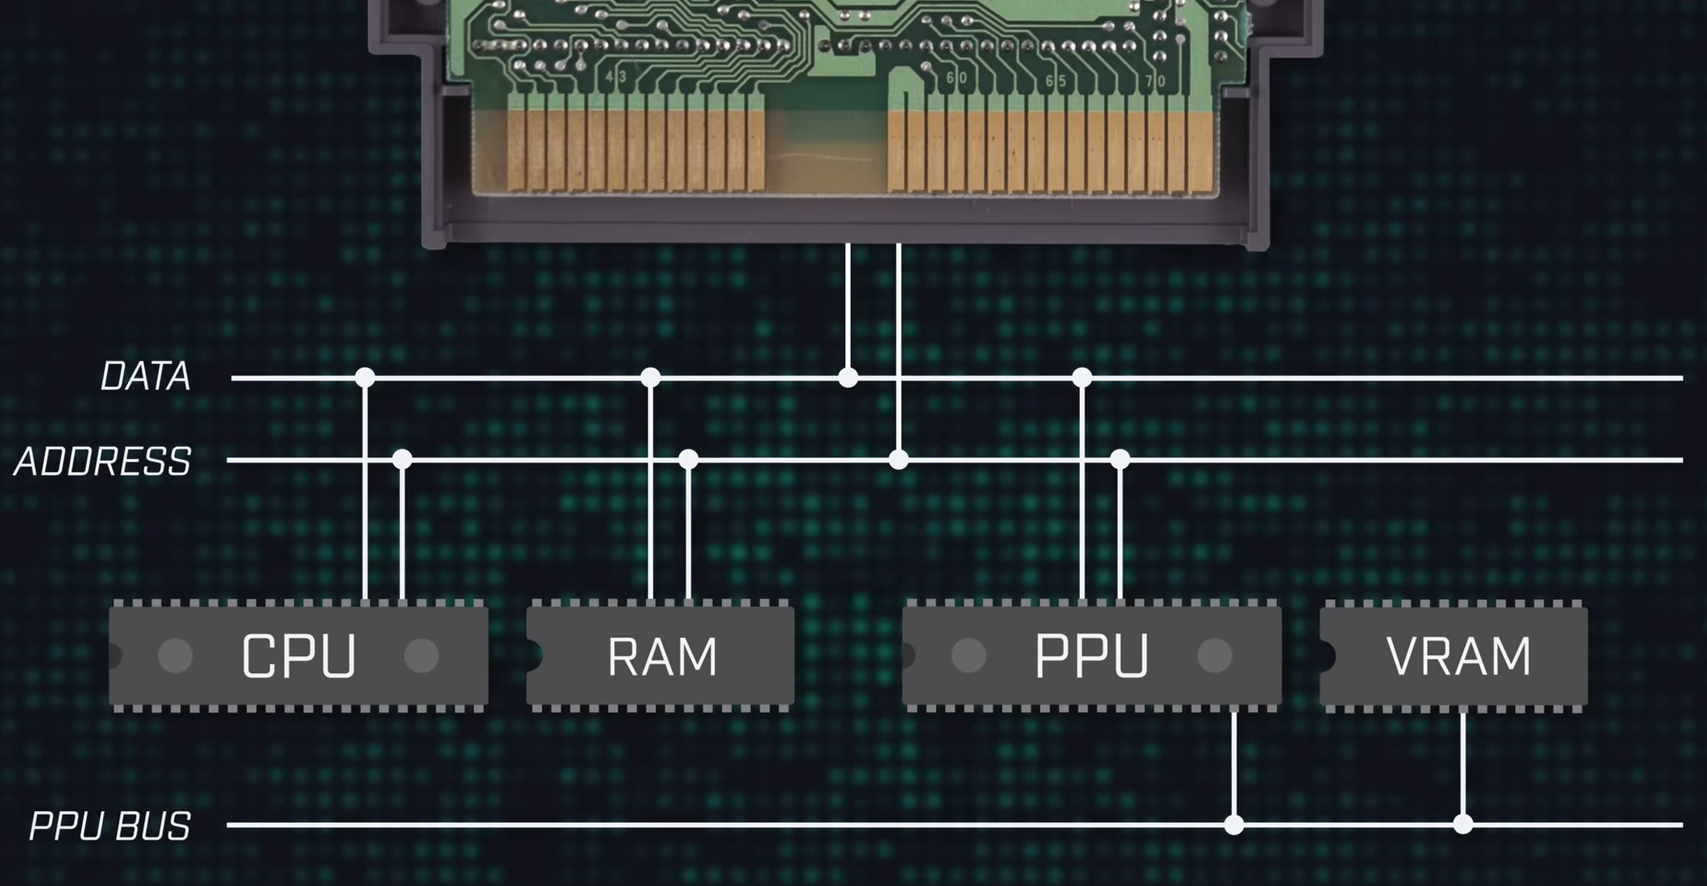
\includegraphics[width=150mm, keepaspectratio]{figures/NES-databuses}
		\caption{Komponensek közti kapcsolat (fent játék kazetta) \cite{NES_hardware}}
		\label{fig:NES-Data-Buses}
	\end{figure}
	

\section{Képalkotás - Picture process unit}

A következőkben azt fogom bemutatni, hogy a NES hogyan tárol, dolgoz fel és jelenít meg sprite grafikákat. A Sprite egy 8x8-as pixel csempét jelent, ez a NES képalkotásának alappillére.

A NES főkomponensei közül a Picture Process Unit (későbbiekben PPU) felelős a konzol 8-bit-es grafikájának elő állításáért. A PPU egy a Nintendo által kifejlesztett speciális chip amely a processzor mellett működik, mint egy társprocesszor (co-processor), hasonlóan a napjainkban elterjedt videókártya-processzor pároshoz.

A CPU-tól eltérően a PPU egy előre meghatározott grafikus műveleti parancs sorozatot hajt végre ciklikusan, nem lehet közvetlenül programozni. Saját memóriával rendelkezik
amelyet a CPU képes módosítani, hogy ezzel megváltoztassa a grafika generálását. Ez a memóriaterület a következőképpen négy részre oszlik:

\begin{itemize}
	\item \emph{Pattern táblák:} Az első szekció tartalmazza a pattern táblákat, amelyek a nyers sprite-kép adatokat tartalmazzák az adott játékhoz. Két pattern tábla van a bal oldali és a jobb oldali tábla amelyek mindegyike 64 kilobyte-nyi memória. Együttesen pedig 256 darab 8 x 8 pixeles csempét tárolnak. A memória ezen része általában közvetlenül 
	a játék kazetta karakter ROM vagy RAM chipjére van leképezve.
	\item \emph{Névtáblák (Nametables):} A következő rész a PPU névtábláit tartalmazza, amelyek a háttérgrafikák kialakítására szolgálnak a játékhoz. Ezek 32x30-as raszterben vannak felépítve, a raszter minden egyes eleme egy 8x8 pixeles területet reprezentál a képernyőn. A cellák egyetlen byte-ot tartalmaznak, amely egy csempét címez meg a Pattern táblákban.  
	\item \emph{Paletták (Palettes):} A harmadik rész az aktív szín paletták tárolására szolgál a játékhoz. A PPU képes több mint 50 különböző szín előállítására, de nem tudja az összes színt egyszerre használni egyidejűleg, ehelyett ezt a memória területet arra használják, hogy meghatározzunk nyolc aktív palettát amelyek egyenként négy színt tartalmaznak. Ebből a nyolc palettából, választhatunk színt a pixel-ek megjelenítése során.
	\item \emph{Objektum Attribútum Memória (későbbiekben OAM):} A PPU memóriának ez a része vezérli a játék előtérben lévő grafikájának megjelenítését. Ezek olyan dolgok, mint például Mario, Link, az ellenségek és az olyan effektek, mint a tűzgolyók és robbanások. Alapvetően bármi, ami a háttér grafika felett vagy néha alatta jelenne meg.
\end{itemize}

Tehát, mindezt összegezve, úgy tekinthetjük a PPU-ra, mintha ez a négy jól elkülöníthető memória terület irányítaná ezt a segéd processzort. A Pattern táblák határozzák meg a nyers képadatokat. A névtáblák határozzák meg a háttér generálását. A színpaletták határozzák meg a használandó színeket és az OAM vezérli az előtérbe vagy háttérbe kerülő mozgó sprite-okat.
Ezen felül a PPU további funkciókkal is rendelkezik, ezeket nyolc különböző regiszter írásával és olvasásával érhetjük el. Ezekről a regiszterekről az implementálás során \aref{sec:PPU-FPGA} fejezetben még olvashatunk.

	\subsection{PPU által generált kimeneti jel}
	\label{subsec:PPU-CRT}
	Ebben a fejezetben bemutatom a PPU által generált jelet és ennek felhasználást a régi típusú CRT TV-kben. A CRT televízió (az eredeti TV) a modern lapos képernyők előfutára volt, alapvetően két fő komponensből épültek fel egy fluoreszkáló képernyőből és egy katódsugárcsőből. 
	
	A CRT működése röviden: a katódsugárcső egy pisztolyként funkcionál, amely elektronokat lő ki a képernyőre és amikor elég elektron találja el a képernyő egy bizonyos területét az világítani kezd. A televíziók kétféle típusban léteztek, fekete-fehérben vagy színesben. A fekete-fehér esetben egy elektronágyú szabályozta a képernyő pixeljeinek monokróm fényerejét, a színes esetben három különálló elektronágyú szabályozta a vörös, kék és zöld komponensek arányát, ezzel megalkotva a színes képet. A színes TV-k esetében is a három elektron sugár együtt mozgott végig a képernyőn, ezért a könnyebb megértés érdekében érdemes egy elektron sugárként gondolni ezekre. 
	
	A televízió működése során a bal felső sarokból kezdve úgy irányítja az elektron sugarat, hogy a teljes képernyőn végigfusson sorról sorra, amíg el nem éri a jobb alsó sarkát a képernyőnek. Ha egy sor végére érünk akkor az elektron sugarat vissza pozicionáljuk a sor elejére, ezt az időt horizontális szinkronizációnak nevezzük (horizontal blanking). Ha végigértünk egy képkockán a TV a katódsugárcsövet újra a felső sor bal oldalára állítja, ezt vertikális szinkronizációnak (vertical blanking) hívják. Ez képalkotási ciklus a TV működése közben rögzített időközönként ismétlődik, általában másodpercenként hatvan képkocka körül. 
	
	%TODO ábra a CRT monitor képalktásáról
	\begin{figure}[H]
		\centering
		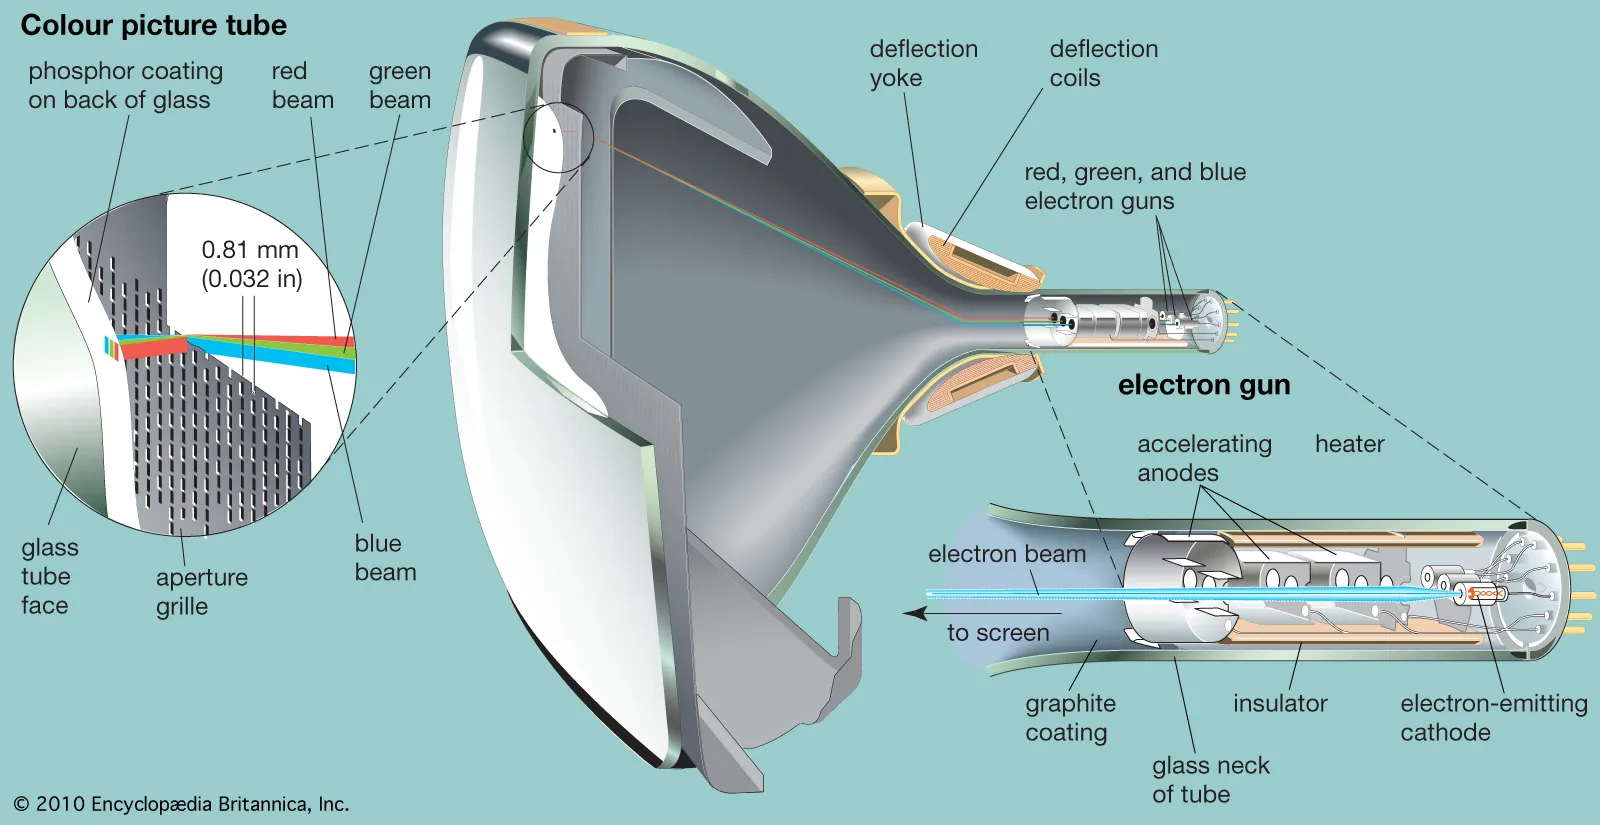
\includegraphics[width=150mm, keepaspectratio]{figures/CRT-TV}
		\caption{Katódsugárcsöves TV-k működése}
		\label{fig:CRT-TV}
	\end{figure}
	
	Miközben a elektronágyú mozog, a TV egy belső jel segítségével tudja szabályozni az elektronok kibocsátásának mértékét. Ez a jel megváltoztatja a szín fényerejét egy adott pozícióban (pixel-en), a pisztoly gyors mozgásának következtében, az eredmény egy folytonos animált kép képernyőn. Ezt a jelet kompozit jelnek nevezzük és általában egy rf antennáról vagy egy kábel dobozból származott, de a NES esetében ezt a jelet a PPU állítja elő. 
	
	A NES két típusú kompozit jelet tudott előállítani, attól függően, hogy a világ melyik területére gyártották. Ez azért következett be mert a CRT TV-knek két standard típusa terjedt el világszerte az NTSC és a PAL. Az NTSC-t elsősorban az Egyesült Államokban és Japánban használták, és 60 képkocka/másodperces sebességgel jelenítette meg kompozit jelet, ezek a TV-k összesen 525 képsorral rendelkeztek. A PAL-t elsősorban Európában, Afrikában és Dél-Amerikában használták és 50 képkocka/másodperc sebességgel futott, összesen 625 képsort jelenített meg.
	
	A NES játékokat sosem programozták régió specifikusak, az egyetlen dolog ami változott területenként az a NES PPU-jának hardvere. Így a világ különböző területein ugyanaz a játék gyorsabban illetve lassabban futott, ez akár 17\%-os különbséget is jelenthetett. A NES emulálás szempontjából az NTSC készülékeket veszem alapul mivel ezeken gépek működését tárták fel részletesebben reverse engineering-gel.
	
	\subsection{Pattern táblák és paletták}
	A sprite képek, amelyek a PPU Pattern tábla memóriájában helyezkednek el, képezik az alapját minden grafikái megjelenítésnek. Ezek a  8 x 8 pixeles csempék alkotják a bonyolult háttereket, mozgó objektumokat és speciális effekteket. Alapvetően a sprite-ok tárolása hasonló módon történik mint egy modern számítógépek által használt kép esetében, mint például png. Mindkét tárolási formátumot kétdimenziós szám rácsként tudjuk elképzelni, ahol minden egyes cellához tartozó érték egy pixelhez tartozó színt reprezentál, csak amíg a png több millió színt támogat addig a NES egy pixel-e csupán négy különböző színű lehet. Gyakorlatilag egy ilyen csempe nem is tárol szín adatokat, a pixel-eket reprezentáló számértékek referenciák egy éppen aktív szín paletta színére.
	
	\begin{figure}[H]
		\centering
		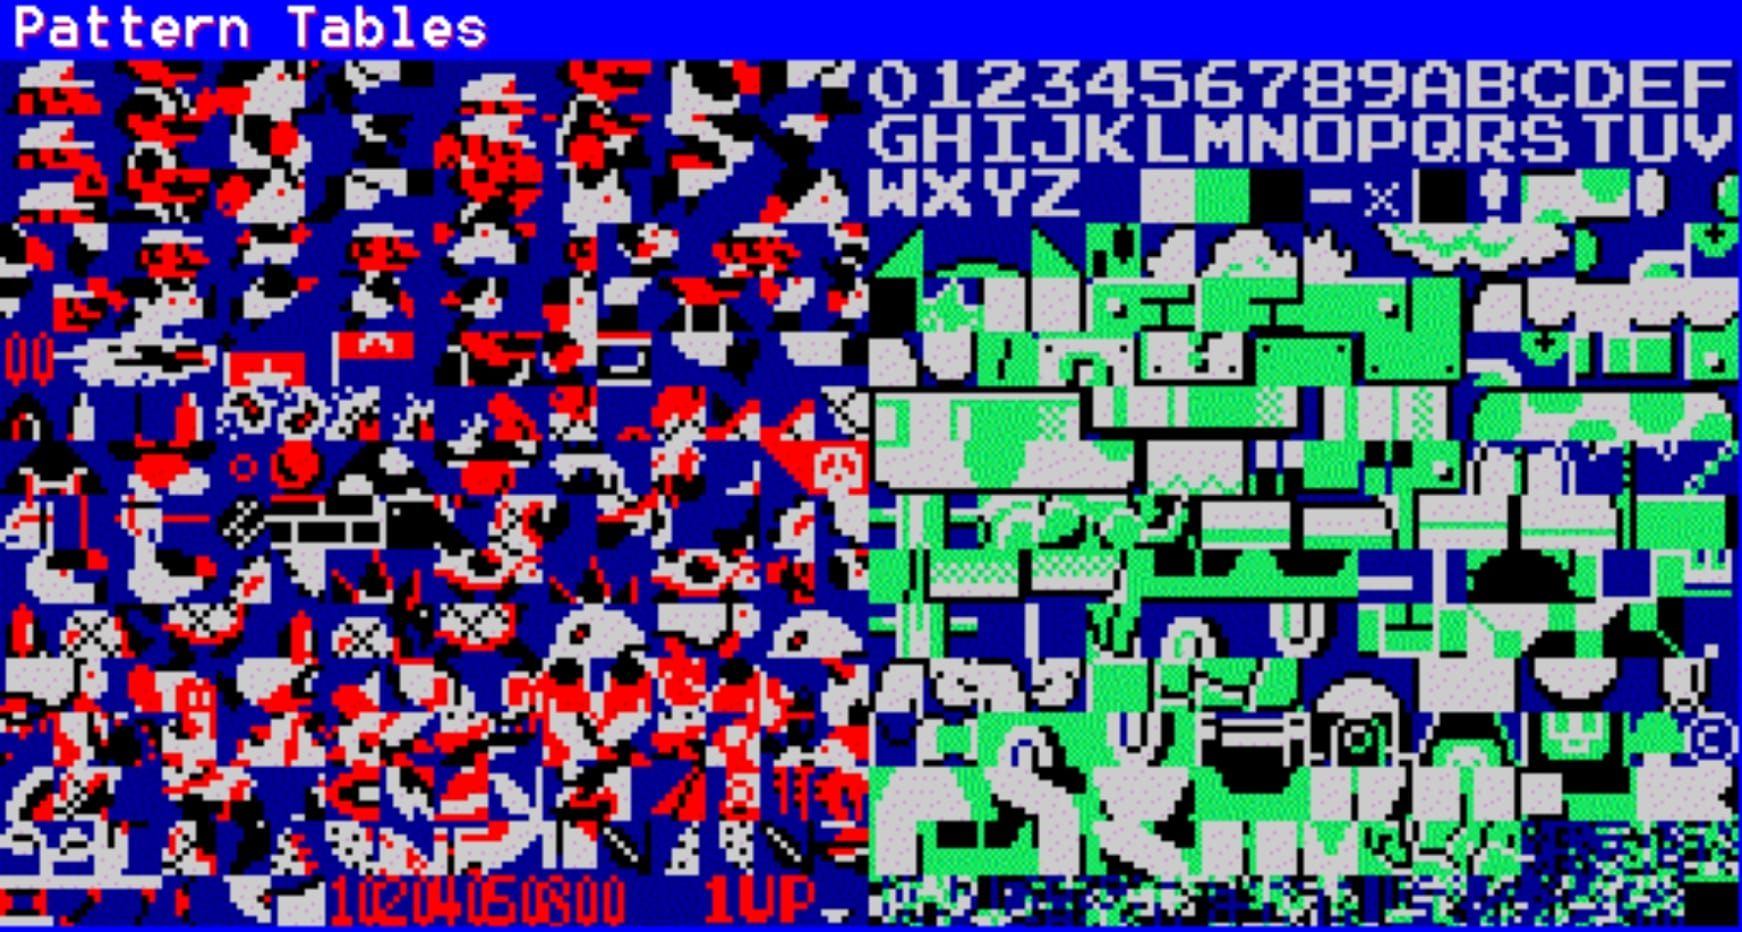
\includegraphics[width=150mm, keepaspectratio]{figures/Mario-Patterns}
		\caption{Super Mario Bros. Pattern táblái}
		\label{fig:Mario-Pattern}
	\end{figure}
	
	A színpaletták memória területének írásával, nyolc különböző palettát állíthatunk be a grafikus megjelenítéshez, négyet a háttér megjelenítéséhez és a maradék négyet az előtér rendereléséhez. Minden egyes paletta négy színt tárol, az első szín minden egyes palettán egy átlátszósági szín, ez azt jelenti, hogy ha a pixel szín értéke nullás indexel rendelkezik akkor az megjelenítés során minden esetben átlátszó lesz (függetlenül a palettába írt szín értéktől).
	
	\begin{figure}[H]
	\centering
	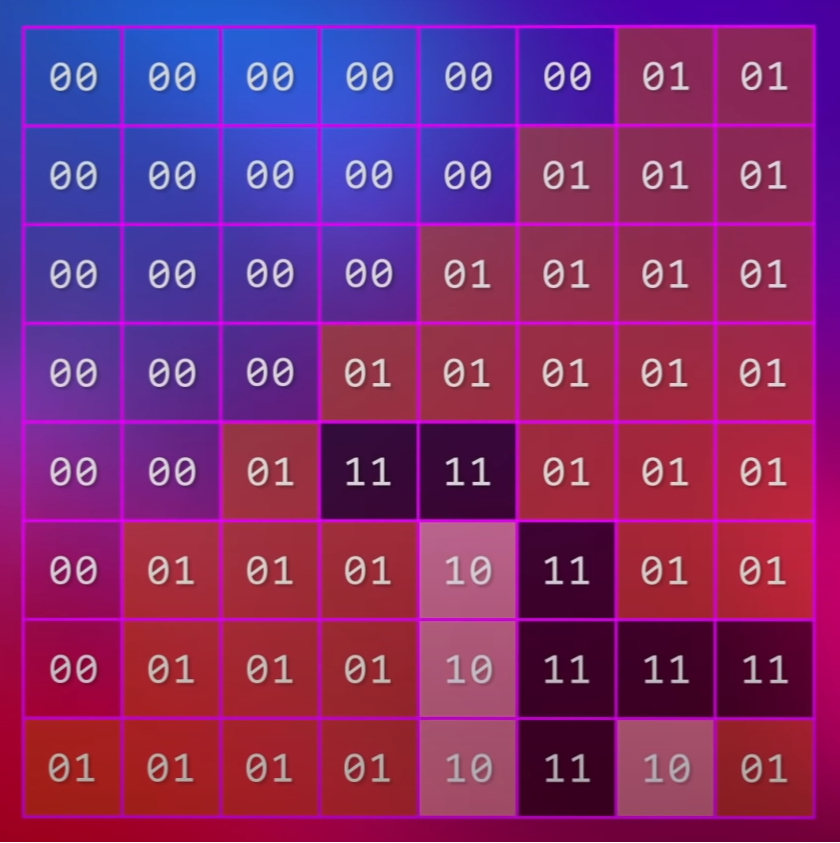
\includegraphics[width=100mm, keepaspectratio]{figures/Gumba-tile}
	\caption{Gumba (Mario egyik ellenfele) bal felső csempe elem szín adatai \cite{Neshacker_ppu}}
	\label{fig:Gumba-tile}
	\end{figure}
	
	A fentiek alapján, tehát egy pixel 0-3-ig vehet fel értéket, tehát 2 biten vagyunk képesek eltárolni az értékét. Egy 8 x 8 as csempe pedig 64 pixelt tartalmaz, ezért összesen 16 byte helyet foglal. Mivel a NES processzora egy 6502-es (8 bit-es) modell volt, ennek okán a legkisebb memóriaegység amit képes volt megcímezni az egy byte volt, így a csempe adatok ésszerű tárolásához egyedi megoldásra volt szükség.
	
	Mivel a NES nem képes direkt a 2 bit-es számértékekkel dolgozni, ezért ezeket fel daraboljuk először logikailag magas és alacsony bitekre. Ezt követően elsőként a csempe alacsony 8 byte-ját tároljuk el majd ezt követően a magas nyolc byte-ot, így megkapjuk a fentebb kiszámolt 16 byte-os értéket. Ezáltal könnyel elérhetővé tettük a kép adatainkat a cpu számára, illetve a PPU-is helyesen képes ezeket megjeleníteni.
	
	\subsection{A név táblák (Name Tables) és tulajdonság táblák (Attribute Tables)}
	
	A név táblák alapvetően, ahogyan már fentebb olvashattuk egy-egy 32 x 30-as rácsként képzelhetők el, ahol minden egyes cella egy csempének felel meg (8 x 8 pixel). Ebből következően egy név tábla 256 x 240 pixelt tartalmaz, ez a CRT monitorok teljes képernyő területe. Egy rács elem, pedig egy, egy byte-os címet tartalmaz, amely az éppen aktív pattern tábla egy csempéjét címzi meg (mivel összesen 256 aktív csempénk lehet ezért elég egy byte a címzéshez).
	
	Ahhoz, hogy a PPU-nk képes legyen egy játék során gyors és gördülékeny háttér változásokra több különböző eszközt fejlesztettek ki. Kezdve azzal, hogy a NES hardveren belül két név táblát helyeztek el, ezek okos címzésével és a hardver sajátosságainak kihasználásával (mirroring) képesek vagyunk az úgynevezett görgetés (scrolling) megvalósítására. Ez egyszerűen egy vertikális vagy egy horizontális finom lapozásnak írható le (egy-két sor pixel eltolásával, illetve megjelenítésével). Alapvető esetben a NES játékok vagy fix háttérrel rendelkeztek (lásd donkey kong), vagy csak horizontális vagy vertikális görgetést alkalmaztak (horizontális - Super Mario Bros.). Viszont a későbbiekben megjelentek komplexebb játékok is amelyek ezek vegyítését alkalmazták ilyen például a Metroid vagy a Legend of Zelda.
	
	A mirroring az a jelenség, amikor két cím azonos memória területre mutat, ez azért fordulhat elő, mert a PPU nem teljes címzést használ (kevesebb bit-tel címez meg tartományokat). A név táblák esetében például egy 2 x 2-es rácsot szoktak képezni ennek segítségével, így kiterjesztve a két névtáblánk címzési tartományát. De ez a jelenség ez egész PPU memória felépítése során megfigyelhető.
	
	%todo memória map
	\begin{table}[H]
		\footnotesize
		\centering
		\begin{tabular}{|l|l|l|}
			\hline
			\rowcolor[HTML]{C0C0C0} 
			\multicolumn{1}{|c|}{\cellcolor[HTML]{C0C0C0}\textbf{Memórai címek}} & \multicolumn{1}{c|}{\cellcolor[HTML]{C0C0C0}\textbf{Méret}} & \multicolumn{1}{c|}{\cellcolor[HTML]{C0C0C0}\textbf{Leírás}} \\ \hline
			$0000 - $0FFF                                                        & \$1000                                                      & Pattern tábla 1                                              \\ \hline
			$1000 - $1FFF                                                        & \$1000                                                      & Pattern tábla 2                                              \\ \hline
			$2000 - $23FF                                                        & \$0400                                                      & Név tábla 1                                                  \\ \hline
			$2400 - $27FF                                                        & \$0400                                                      & Név tábla 2                                                  \\ \hline
			$2800 - $2BFF                                                        & \$0400                                                      & Név tábla 3                                                  \\ \hline
			$2C00 - $2FFF                                                        & \$0400                                                      & Név tábla 4                                                  \\ \hline
			$3000 - $3EFF                                                        & \$0F00                                                      & A $2000 - $2EFF címterület mirror-ja                         \\ \hline
			$3F00 - $3F1F                                                        & \$0020                                                      & Szín paletta RAM indexek                                     \\ \hline
			$3F20 - $3FFF                                                        & \$00E0                                                      & A $3F00 - $3F1F címterület mirror-ja                         \\ \hline
		\end{tabular}
		\caption{A PPU memória kezelése (14 bit címek) mirroring jelenséggel}
		\label{tab:PPU-memory}
	\end{table}
	
	Minden egyes névtábla végén egy kisebb extra memória terület található, amelyet tulajdonság táblának (vagyis Attribute Table-nek) nevezünk. Ez egy kisebb táblázatként képzelhető el ahol miden egyes cellában egy byte adatot tárolunk, viszont ennek feloldása bonyolultabb mint névtáblák esetében. Ez a 8 bit egy 4 X 4 csempényi háttér terület szín palettáját határozza meg a következő képen:
	
	\begin{itemize}
		\item az első két bit a bal felső 2 x 2 csempe palettáját határozza meg, 
		\item a második két bit a jobb felső 2 x 2-es terület palettáját határozza meg, 
		\item a harmadik két bit a bal alsó 2 x 2-es terület palettáját határozza meg,
		\item végül pedig az utolsó két bit a jobb alsó terület színérért felelős.
	\end{itemize}
	
	 Így a teljes képünket 8 x 8 ilyen byte-tal írhatjuk le. 
 
 	 \subsection{Objektum Attribútum Memória (OAM)}
 	 Ez a memória terület 64 külön álló sprite tárolására képes. Minden egyes OAM spritehoz négy byte adat tartozik. Az első byte meghatározza a vertikális vagy y koordinátáját a sprite-nak. A második byte azt határozza meg, hogy melyik 8 x 8-as csempe legyen megjelenítve az éppen aktív Pattern táblából. A harmadik byte segítségével különböző tulajdonságait vagyunk képesek befolyásolni a sprite-nak. Végül pedig az utolsó byte a horizontális vagyis x koordinátáját határozzam meg az objektumnak.
 	 
 	 Az előbb bemutatott byte-ok közül az egyetlen bonyolultabb működésű a harmadik, ebben az estben is a különböző bit-ek más és más működést kódolnak.  Az nulladik és az első bit egy előtér szín palettát választanak ki a sprite számára. A következő három bit (3, 4 és 5) nem használtak. Ezt követően az ötödik bit határozza meg, hogy a sprite a háttér elé vagy mögé kerüljön (ha értéke nulla akkor a háttér fölé fog kerülni, ha pedig egy mögé). Végül pedig a hatodik illetve hetedik bitek azt határozzák, hogy a sprite pixel-ei horizontálisan vagy vertikálisan helyet cseréljenek (tükrözve legyenek), nulla esetén a sprite eredeti formájában marad, egy esetén, pedig meg tükröződik. Ez egy nagyon hasznos tulajdonság, hiszen így a játék fejlesztők rengeteg memória területet spórolhattak a Pattern táblákból. Mivel több olyan objektumot, karaktert vagy effektet is tervezhettek amelyek vagy horizontálisan vagy vertikálisan szimmetrikusak voltak (erre az egyik legjobb példa a felvető gomba  a Super Mario Bros. videojátékból).    
 	     
 	 \subsection{PPU hardveres hibái (bug-ok)}
 	 Mivel hardveres emulálást készítünk, ezért nem mehetünk el az eredeti hardver hibái mellett. Az esetek többségében a NES játékok fejlesztői kihasználták ezeket az hazárdokat a játékfejlesztéseik során. Tehát ha az eredeti játékokkal szeretnénk játszani ezekkel is maradéktalanul meg kell ismerkednünk.
 	 
 	 A PPU leghíresebb ilyen hibája, a sprite túlcsordulás kezelése (Sprite Overflow Bug). Ez a OAM feldolgozása és megjelenítése közben alakulhat ki a NES-ben. Ennek megismeréséhez először is érdemes áttekinteni, hogy a PPU milyen állapotgép alapján dolgozza fel a OAM-ot. A PPU-n belül található egy másodlagos OAM amely nyolc sprite eltárolására képes, ennek a nyolc sprite-nak a megjelenítése történik a NES egy 256 pixeles sorban. Minden egyes sorral ebbe a memória területbe töltjük be az éppen aktív sprite-okat, ennek következtében a 64 sprite közül csupán nyolcat tudunk egy sorba megjeleníteni. Ezek alapján az OAM megjelenítés a következő négy lépésből áll:
 	  
 	 \begin{enumerate}
 	 	\item először is megtisztítjuk a másodlagos OAM-ot,
 	 	\item majd végigvizsgáljuk a teljes OAM-ot és kiválasztjuk azokat a sprite-okat amiket a következő sorban meg kell jeleníteni (ezekből az első nyolcat),
 	 	\item ha a megtaláltuk a 8 megjelenítendő sprite-ot akkor sajnos egy hibás implementációval végig vizsgálja az eszköz, hogy van-e még aktív sprite a sorban (ha talál ilyet beállítja a Sprite Overflow Flaget),
 	 	\item végül pedig a PPU feltölti a megjelenítéshez szükséges regisztereket az éppen aktív spritok adataival.
 	 \end{enumerate}
 	 
 	 A következő sorban megjelenítendő aktív sprite-ok kiválasztása, az objektumok y értéke alapján történik az OAM-ban tárolt prioritási sorrend alapján. A fent említett rendszerhiba a harmadik lépésben következhet be, amikor a PPU megtalálta a nyolcadik sprite-ot, ezt követően elkezdi vizsgálni a maradék OAM területet, viszont ennek vizsgálata csak az első esetben következik be helyes tulajdonság szerint (y érték). Ezt követően a a sprite-ok tulajdonságaiban diagonálisan haladunk (tehát a második keresés a Pattern tábla cím alapján történik, és későbbiekben így tovább halad az objektum négy byte-ján keresztül), így olyan esetben is bejelezhet a sprite túlcsordulást jelző flag (Sprite Overflow Flag), amikor ez nem is történt meg. Erre a hibára több híres játék is épített az egyik leghíresebb a The Legend of Zelda, de például a Ninja Gaiden és Castlevania sorozatokban is meg jelent.
 	 
 	 Egy másik kevésbé ismert hazárd az OAMADDR regiszterrel kapcsolatban találtak meg. Ez általában akkor jött elő amikor nem a DMA vezérlőt használták az OAM frissítésére, hanem a szimpla byte elérését. Ilyenkor néha elő fordult, hogy egy egy bájtot rossz OAM területre másolt az eszköz, ezzel beszennyezve az OAM-ot. Ennek a bug-nak későbbi kompatibilitási okai voltak.    
 	 
 	       
\section{2A03 a NES fő vezérlő egysége}

A NES videojáték konzol egy komplex több feladatot ellátó fő végrehajtó egységgel rendelkezik, melynek neve 2A03 (RP2A03[G] NTSC konzolokban). A chip három fő hardveres elemből áll. Először is a kor legjobban elterjedt CPU-jának a MOS 6502-esnek egy módosított változatát tartalmazza, emellett helyet kap még az APU társprocesszor (co-processzor) is, amely a hang generálásért felelős végrehajtó egység, illetve az adatok gyorsabb másolását elősegítő DMA egységet. A következőkben ezt a három hardvereset elemet ismerhetjük meg kicsit részletesebben.

	\subsection{MOS 6502 - központi feldolgozó egység (Central Processing Unit, CPU)}
	
	A CPU alapja a MOS Technology 6502-es 8 bites architektúrával rendelkező mikroprocesszora. A processzort Chuck Peddle és Bill Mensch amerikai mérnökök tervezték és először 1975-ben mutatták be. Már a kezdetektől nagy sikernek számított kompakt és egyszerű designja és jó programozhatósága miatt. Egyszerűsége miatt sokkal kevesebb tranzisztorban elfért (3510 tranzisztor) mint vetélytársai az Intel és Motortollától. Anyagköltsége miatt nagyon kedvező áron kezdhették el forgalmazni (csupán 25 dollár). A leghíresebb felhasználásai az Apple 1, 2, illetve a Commodore 64. Több játék konzol is felhasználta a chip architektúráját saját CPU-ik kialakításához (NES, SNES, Atari 2600). 
	
	A processzor egy órajel bemenettel rendelkezik $\phi0$, amelyet a NES esetén egy külső kvarc kristály hajt meg 1.789773 MHz frekvencián (\ref{fig:NES-Motherboard}). Ebből a beérkező órajelből állít elő a processzor két, eltolt fázisú órajelet $\phi1$ és $\phi2$. Ezzel több szinkronizációs lehetőséget engedve egy órajelenbeliül a külső hardvereknek. A 6502 8 bites architektúrája azt jelenti, hogy a processzorunk egy byte adatot képes feldolgozni/módosítani egy órajel lefutása alatt.Tehát 8 bites adatbusszal és egy 16 bites címbusszal rendelkezik. Az 2A03-as modellekben a Nintendo mérnökei annyiban módosították az eredeti MOS architektúrát, hogy letiltották a cpu decimális módját.

	\begin{figure}[H]
	\centering
	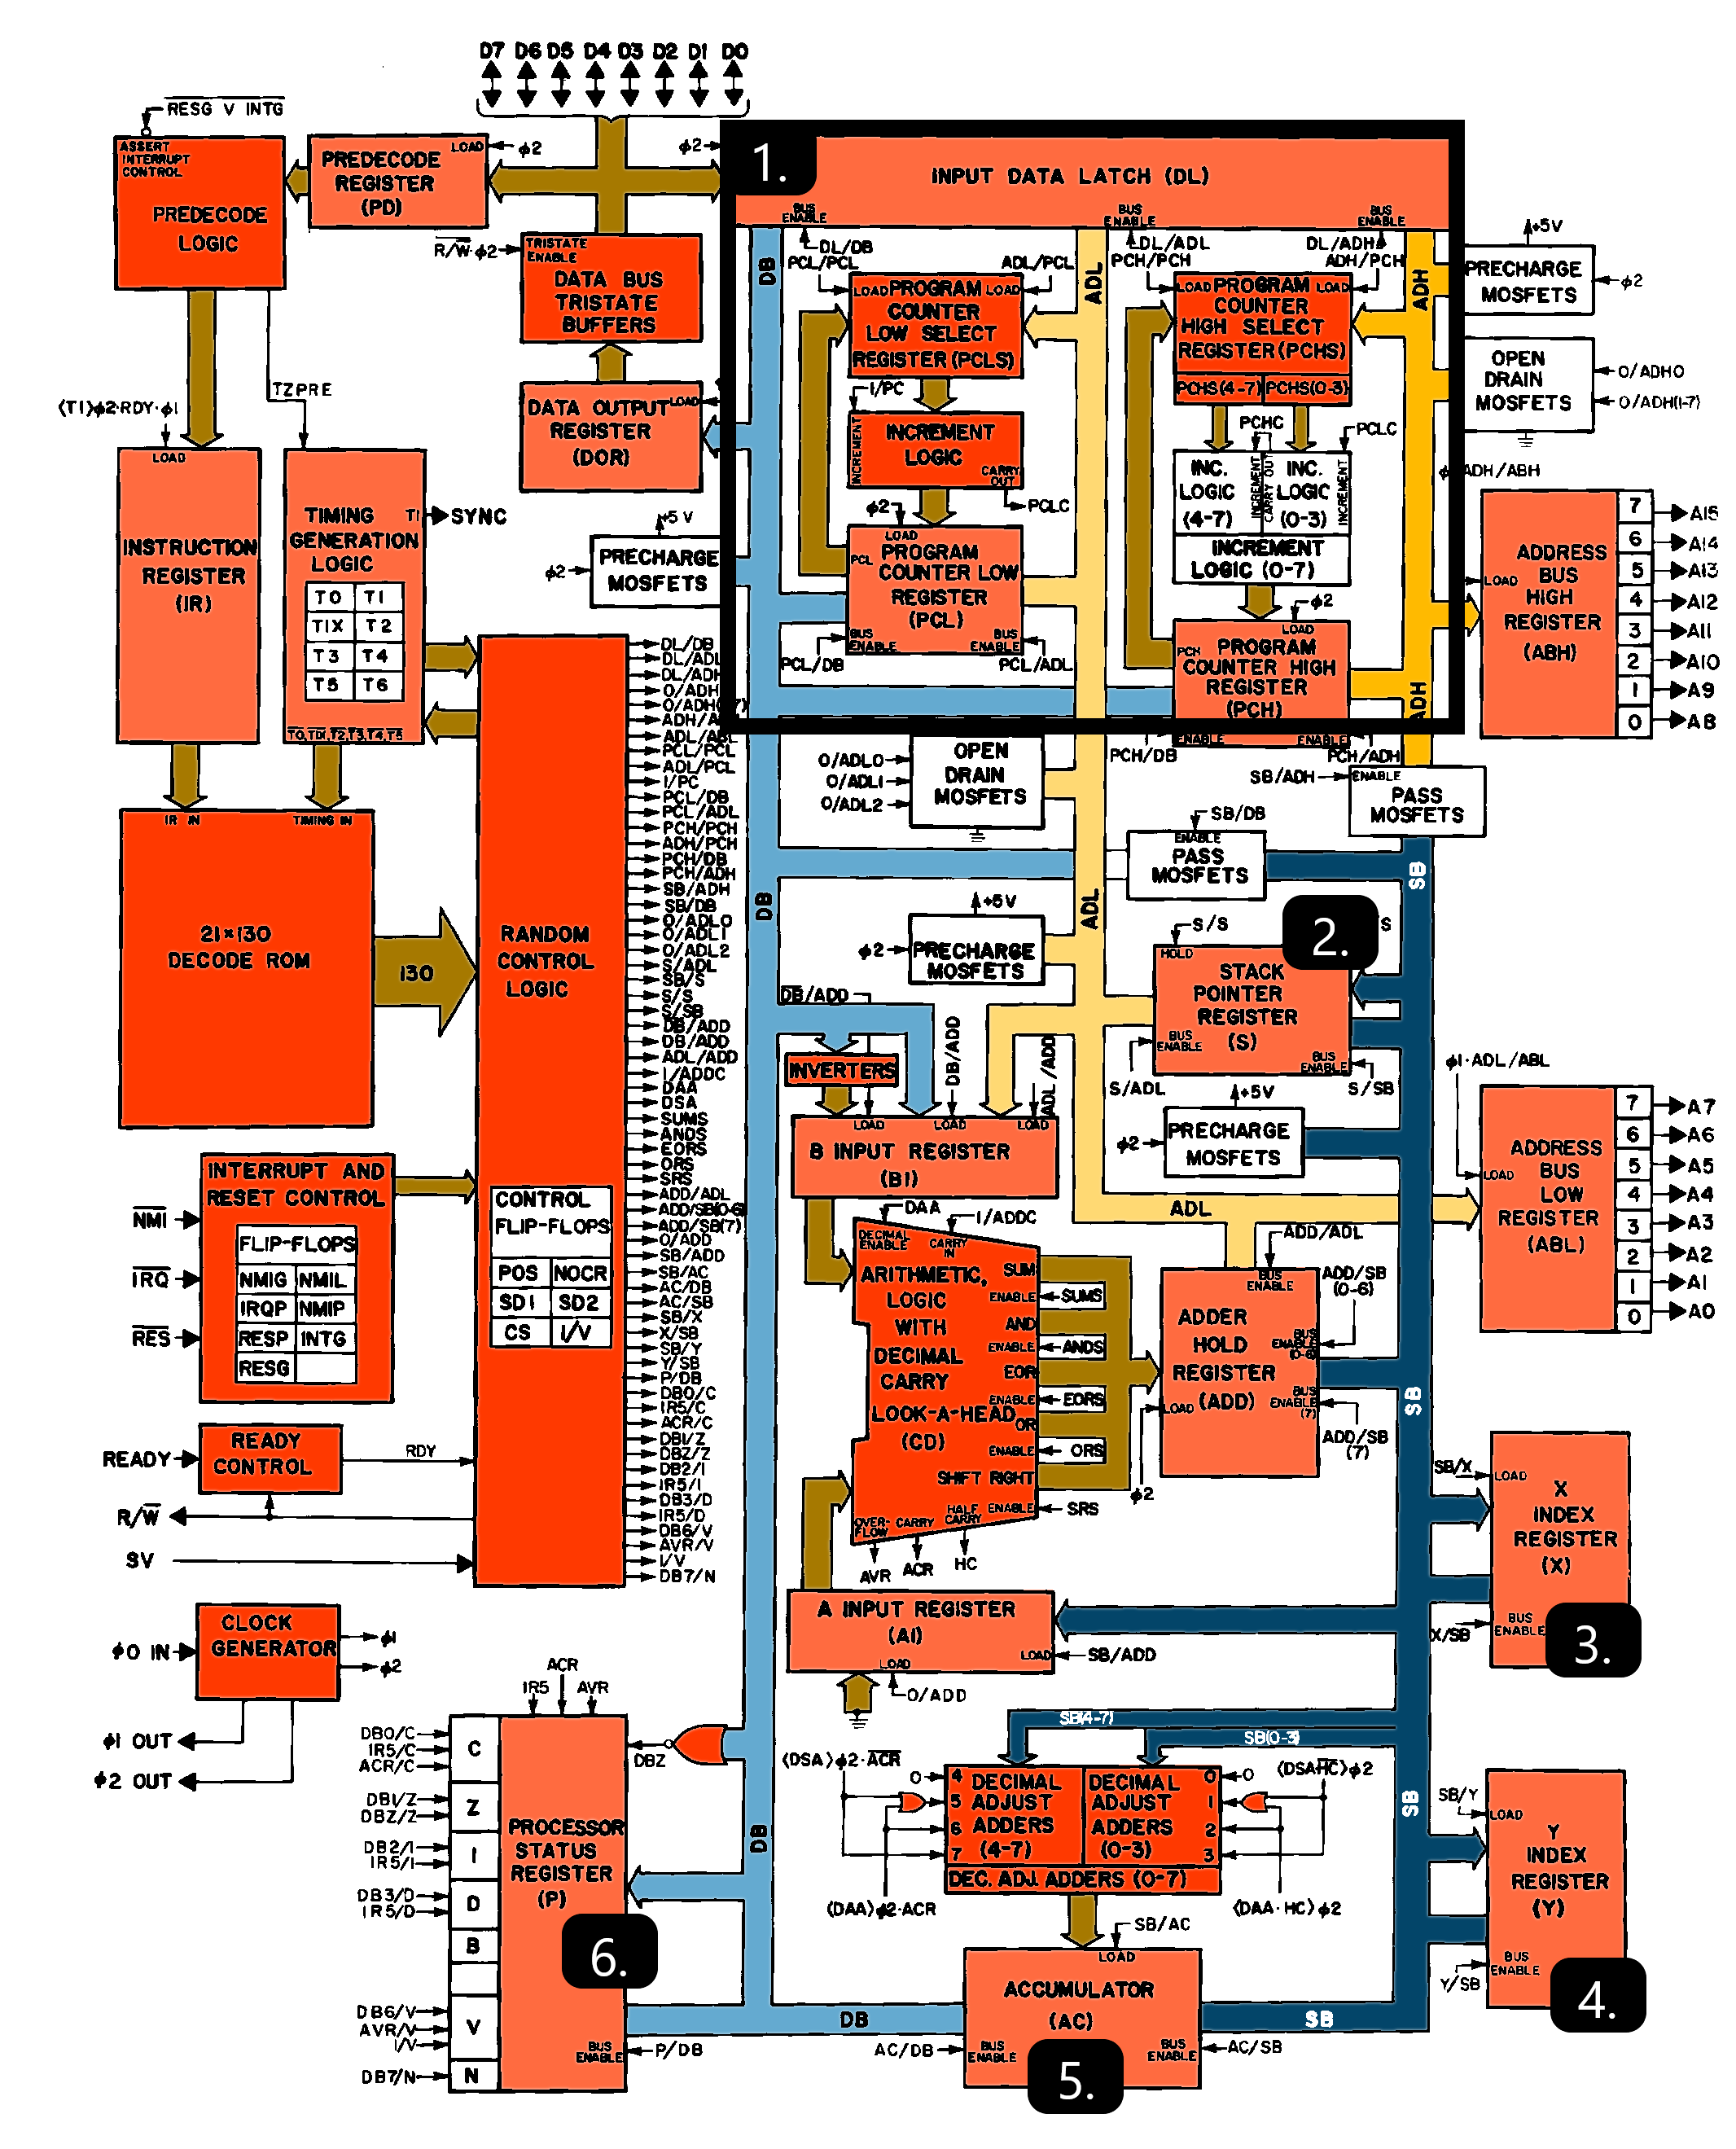
\includegraphics[width=150mm, keepaspectratio]{figures/6502-blokk-diagram-pined}
	\caption{A MOS 6502 egyedi nyolcbites architektúrája}
	\label{fig:6502-Blokk-diagram}
	\end{figure}

	A 6502 8 bites architektúrája hat regiszterrel rendelkezik. Ebből három (A, X, Y) általános programozási célokat tölt be. Három pedig speciális belső információk tárolására szolgál (PC, SP, SR). Ezek elhelyezkedését és logikai kapcsolatát láthatjuk \aref{fig:6502-Blokk-diagram} képen.
	
	\begin{enumerate}
		\item \emph{Program számláló (Program Counter, PC):} 16 bites regiszter, amely a program jelenlegi címét tartalmazza (ennek a regiszternek a mérete határozza meg a cím tartományt)
		\item \emph{Verem mutató (Stack Pointer, S):} 16 bites regiszter, viszont felső nyolc bitje fix decimális egy (0000 0001) értékkel rendelkezik. Tehát valójában egy 8 bites regiszter, amely a verem aktuális címére mutat. 
		\item \emph{X index regiszter:} 8 bites index regiszter programozás során fölfelé és lefelé is számolhatunk vele. Általában adat indexelésre használjuk, de aritmetikai művelet is végrehajtható rajta.
		\item\emph{Y index regiszter:} 8 bites index regiszter használata megegyezik a az X index regiszter használatával. 
		\item \emph{Akkumulátor (Accumulator, A):} 8 bites regiszter fő szerepe az adat tárolás, ha bármilyen műveletet végzünk a processzoron annak eredménye ebben a regiszterben kerül eltárolásra.
		\item \emph{Processzor Státusz Regiszter (P):} 8 bites regiszter, a processzor státusz flagjeit tárolja \aref{fig:6502-P-reg} ábrán látható módon.	
	\end{enumerate} 
	
	\begin{figure}[H]
		\centering
		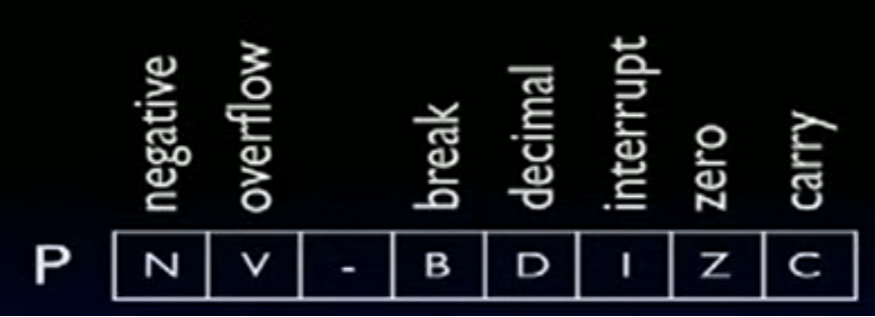
\includegraphics[width=100mm, keepaspectratio]{figures/6502-P-reg}
		\caption{A MOS 6502 processzor státusz regisztere (P)}
		\label{fig:6502-P-reg}
	\end{figure} 
	
	opkódok
	
	memória cím tartomány

	\subsection{Audió feldolgozó egység (Audio Process Unit, APU)}
	
	5 sound chanel

	\subsection{DMA}
	
	sprite/ dmc mode

\section{NES joypad}
